\documentclass[11pt]{article}

\usepackage[margin=1in]{geometry}
\usepackage{amsmath}
\usepackage{amssymb}
\usepackage{graphicx}
\usepackage{booktabs}
\usepackage{hyperref}
\usepackage[style=apa,backend=biber]{biblatex}
\addbibresource{references.bib}

\graphicspath{{output/graphs/}}

\title{Human in the Loop: AI Exposure and Labor Market Frictions\\
       \large (Excerpt of Empirical Section)}
\author{Leyao Wang\\ \small University of Virginia}
\date{}

\begin{document}
\maketitle

\section*{Introduction}

The public release of ChatGPT in November 2022 marked a turning point in the diffusion of generative AI.  Within months, firms and workers began adopting generative AI tools to perform a growing range of tasks: drafting emails, writing code, summarizing documents, analyzing data.  When a new technology performs tasks that workers are paid to do, the net effect on their wages and employment is not obvious \emph{a priori}: it depends on whether the productivity gains that accrue to them, through expanded output and rising demand for tasks complementary to generative AI, are large enough to offset the substitution pressure they bear directly.

This paper uses the Current Population Survey Annual Social and Economic Supplement (CPS-ASEC) for 2018--2025, linked to the occupation-level AI exposure scores of \textcite{eloundou2024gpts}, to estimate how generative AI has affected U.S.\ labor-market outcomes in the three years since ChatGPT's release.  The excerpt that follows reproduces the data, empirical strategy, and main wage-result sections of the full thesis; the thesis itself additionally develops a task-based toy model, reports unemployment and heterogeneity results, and discusses the mechanisms behind an education-asymmetric wage compression finding.

\section*{Data}

The primary data source is the Annual Social and Economic Supplement to the Current Population Survey (CPS-ASEC), accessed through IPUMS \parencite{ipumscps2025}.  The CPS-ASEC is a nationally representative annual survey that captures labor-force status, occupation, wage income, and detailed demographic characteristics for approximately 100,000 households.  I use eight survey waves covering income reference years 2018--2025, spanning both the pre- and post-ChatGPT periods.

\paragraph{Unemployment.} The unemployment indicator equals one if a respondent is classified as unemployed by the CPS --- not working but actively searching for work (CPS \texttt{empstat} codes 21 and 22) --- and zero otherwise.  The sample mean is 3.4\%, roughly consistent with official U.S.\ unemployment statistics over this period.

\paragraph{Wages.} For the wage analysis, I use annual real wage and salary income (\texttt{incwage}), deflated to 1982 dollars using the annual average CPI-U from FRED \parencite{fred_cpiaucsl}.  The outcome variable is the natural log of real wages.  Observations with zero or missing wage income are excluded from the wage sample (workers who are unemployed or out of the labor force for wage purposes), yielding 464,300 observations.

\paragraph{AI exposure.} The AI exposure variable is drawn from \textcite{eloundou2024gpts}, which constructs occupation-level LLM exposure scores from the O*NET 27.2 database.  Annotators rate each task on a three-category rubric (no exposure, direct exposure, LLM-augmented exposure), and the occupation-level score $\beta_o$ aggregates these ratings with partial weight on LLM-augmented tasks.  After a hierarchical crosswalk from Census occupation codes to 2018 SOC codes, the resulting $\beta_o$ is time-invariant and assigned at the occupational level.  In the CPS-ASEC worker-year sample, $\beta_o$ has a mean of $0.37$ and a standard deviation of $0.21$, ranging from $0$ to $0.98$.

\section*{Empirical Strategy}

The core empirical question is whether outcomes for workers in high-exposure occupations moved differently from outcomes in low-exposure occupations after ChatGPT's release, relative to how they moved before.  The estimating equation is:
\begin{equation}
\label{eq:main}
Y_{it} = \alpha
  + \sum_{t \neq 2022} \beta_t \left( \mathbf{1}[t] \times \text{AIExposure}_i \right)
  + \text{lower-order terms} + X_{it}'\Gamma + \varepsilon_{it},
\end{equation}
where $Y_{it}$ is either the unemployment indicator or log wages for worker $i$ in year $t$; $\text{AIExposure}_i$ is the worker $i$'s occupation's AI exposure score; and year 2022 is the omitted category.  The lower-order terms include year fixed effects and the main effect of AI exposure.  The $\beta_t$ coefficients trace, year by year, whether high-exposure workers diverge from low-exposure workers relative to the 2022 baseline.  If AI caused labor-market disruption after its diffusion, we expect the post-2022 $\beta_t$ to be positive (for unemployment) or negative (for wages), while the pre-2022 $\beta_t$ should hover near zero.

Four progressively stricter specifications are estimated: (1) no additional controls, (2) sex fixed effects, (3) sex and education fixed effects, and (4) sex, education, and state$\times$year two-way fixed effects.  Specification (4) absorbs state-specific time shocks and is the preferred specification.  Standard errors are clustered at the occupation level across all specifications to address heteroskedasticity and within-occupation correlation in the error term that arises because $\beta_o$ is assigned at the occupation level.

The coefficient $\hat\beta_t$ is interpreted as the per-unit marginal effect of AI exposure on the outcome in year $t$, relative to the 2022 baseline.  \textcite{callaway2024continuous} show that under the continuous-treatment two-way fixed effects specification, this coefficient is a weighted average of the underlying per-exposure effects, with weights that need not reflect the population exposure distribution.  I acknowledge this as a known limitation of the specification.

\section*{Main Wage Result}

Figure~\ref{fig:logwage_stateYFE_plot} plots the event-study coefficients for log real wages in the preferred specification.  Pre-ChatGPT coefficients for 2018, 2019, and 2020 are uniformly small and statistically insignificant across all four specifications, consistent with parallel wage trends.  The 2021 coefficient is positive ($\approx +0.05$) and marginally significant at the 10 percent level in the two specifications that include education fixed effects.  I interpret this as a carryover of the same COVID-recovery asymmetry flagged in the unemployment results, with wages in high-exposure occupations rebounding faster than those of less-exposed occupations as the pandemic receded.  Post-ChatGPT, the wage adjustment is weaker than the unemployment adjustment and emerges only late in the sample.

\begin{figure}[htbp]
\begin{center}
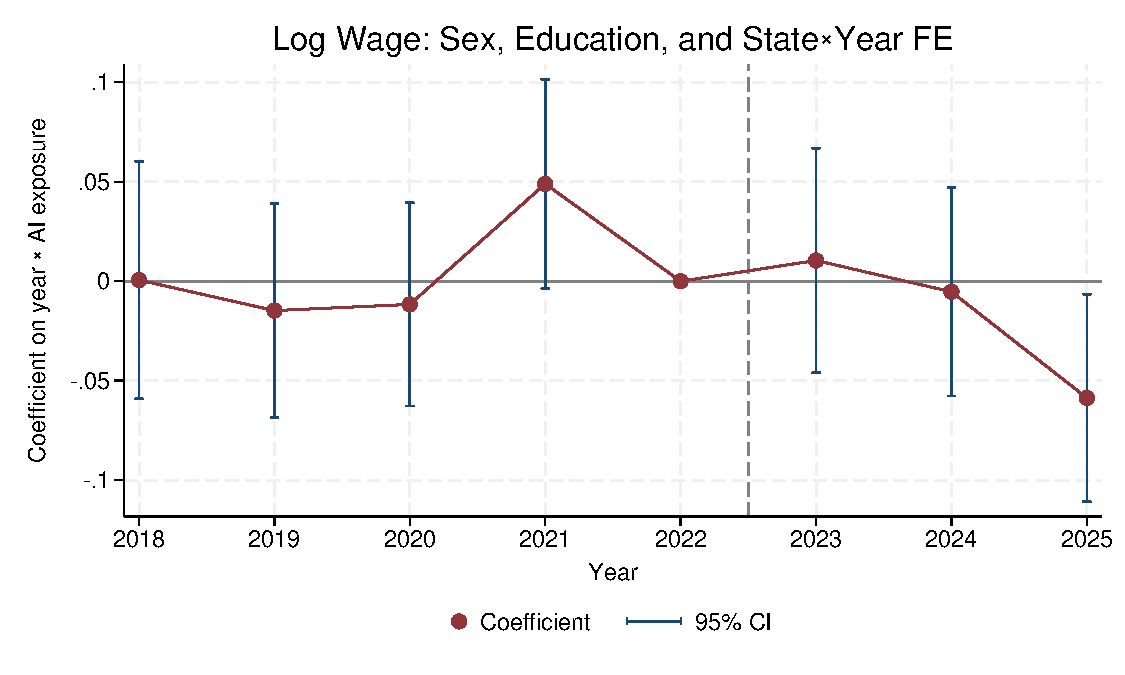
\includegraphics[width=0.8\textwidth]{logwage_stateYFE_plot.pdf}
\caption{Log real wage: DiD coefficients (year $\times$ AI exposure), preferred specification (sex, education, and state$\times$year fixed effects). Year 2022 is the baseline ($\hat\beta_{2022} = 0$). Error bars are 95\% CI, SEs clustered at the occupation level.}
\label{fig:logwage_stateYFE_plot}
\end{center}
\end{figure}

In the naive and sex-FE specifications, the 2025 coefficient is $-0.036$ and $-0.046$ respectively, neither significant at conventional levels.  Only the most demanding specification (absorbing sex, education, and state$\times$year fixed effects) produces a statistically significant 2025 coefficient ($-0.059^{**}$).  No significant effect appears in 2023 or 2024 under any specification.

The delayed wage response is consistent with the displacement channel discussed in the unemployment results: with wages downward-sticky, adjustment flows first through the extensive margin (employment), and the intensive margin (wages) lags behind.

The fact that statistical significance requires state$\times$year fixed effects is itself interesting.  On the one hand, this could suggest a potential weakness of the wage result: the estimate is not robust across all 4 specifications.  On the other hand, this could suggest that noise from region-specific shocks in 2025 may have been large enough to mask the exposure signal in looser specifications.  I note both interpretations as possible and do not strongly favor one over the other.

My second concern is that 2025 is the end of the sample.  Whether the relative difference in wage persists in 2026 is an empirical question the current data cannot answer, given my inability to travel to the future.  I suggest readers to interpret the 2025 result with that uncertainty in mind.

Finally, the 2025 estimate should be interpreted in relative terms.  A negative estimate does not imply that real wages fell in absolute terms for high-$\beta_o$ workers, or indeed that wages fell at all: aggregate wages may have risen uniformly post-2022, and the coefficient would still be negative if they rose by less in high-exposure occupations than in low-exposure ones.  What the estimate captures is the differential wage path along the $\beta_o$ distribution post-2022.

\printbibliography

\end{document}
